The earlier picture of probability and inference can be usefully cast in the language of physics and energy. By leveraging this correspondence, we can import analytic and computational tools from physics to tackle statistical questions. In this section, we will define a physical model of coin flips and demonstrate its equivalence to the statistical model discussed earlier. We will then explore how this perspective motivates alternative types of models and inference techniques. 

Physics often describes systems in terms of a~\emph{configuration space} of possible~\emph{states}.  In the coin flip example, the state of the system (or "configuration") is the sequence of $n$ observed outcomes. We represent this configuration as a vector~$\vec{s}$, where each entry~$s_i = 1$ indicates that flip~$i = 1,...,n$ landed heads, and~$s_i = 0$ represents tails. The configuration space of coin flips is thus comprised of all possible sequences of $n$ flips, forming all binary vectors of length~$n$. 

This notation elicits the \emph{Ising model} fundamental to statistical mechanics. The configurations of this model consist of atomic "spins" that reside at one of~$n$ "sites," each in either its \emph{excited state}~$s_i = 1$ or \emph{ground state}~$s_i = 0$\footnote{The two values of an Ising model spin are typically denoted as~$s_i = 1$ for the "up" state and~$s_i = -1$ for the "down" state, in line with the magnetic dipole moments they physically represent, although the choice of basis does not alter the underlying physics.}. We assign the excited state an \emph{energy} of 1 and the ground state energy 0, as shown in Figure~\ref{fig:coin-flip-energies}. The total energy of the system, referred to as the \emph{Hamiltonian}, is then the number of excited states (or heads) \begin{align}
    H(\vec{s}) = \sum_{i=1}^n \left(0 \delta_{s_i 0} + 1 \delta_{s_i 1}\right) = n_H. \label{eq:coin-flip-energy}
\end{align} 
A more general Ising model would include coupling energies between neighboring spins, but we omit them here to maintain independent coin flips. In Appendix~\ref{app:SBM-Ising} we discuss the deep connections between the more general interacting Ising model and statistical models of network group structure.

\begin{figure}
    \centering
    
\includegraphics{max_dissertation//chapters//figures//chp1/coin-flip-energies.pdf}
    \caption{Physical interpretation of coin flips. Heads ("H") have energy~$E = 1$ while tails ("T") have energy~$E = 0$, so that the overall energy of the configuration~$\vec{s}$ is equal to the number of observed heads,~$H(\vec{s}) = n_H$.}
    \label{fig:coin-flip-energies}
\end{figure}

In an isolated system the energy Eq.~\eqref{eq:coin-flip-energy} is always conserved, a fundamental law of physics. Although changes in individual spin states can occur, they must be counterbalanced by changes in other spins to maintain the "global" energy of the system. Let~$E$ be this constant energy of the system, so that only configurations~$\vec{s}$ where~$H(\vec{s}) = E$ are permitted, cases with~$n_H = E$ excited states. The number of possible system configurations (also known as \emph{microstates}) that satisfy this condition is then the number of ways to arrange the~$n_H = E$ excited states among the~$n$ sites, \begin{align}
    \Omega(E) = \binom{n}{E}. \label{eq:Omega-E}
\end{align}

Statistical mechanics fundamentally postulates that when a system is in~\emph{equilibrium}, all these microstates of the same total energy are equally likely to appear. This assumption defines equilibrium statistical mechanics, the framework we adopt in this thesis. Under this postulate the probability of observing any specific configuration~$\vec{s}$ is therefore \begin{align}
    P(\vec{s}|E) = \binom{n}{E}^{-1}. \label{eq:coin-flip-P-microcanonical}
\end{align}
This uniform distribution over all configurations of a fixed energy is known as the~\emph{microcanonical ensemble}. As a distribution over possible sequences of coin flips, it can also be interpreted as a~\emph{microcanonical model} where the continuous local probability of heads~$p$ has been replaced by the discrete global number of heads~$n_H = E$. 

Many of the statistical models we consider in this thesis are framed in this microcanonical form, where the "parameters" are globally observed quantities. While this formulation may not be well-suited for the coin flip example, where we have little reason to expect a "conservation of heads," it arises in other statistical settings where certain properties are conserved across random realizations. For instance, in a network of sports matches the total number of games played each season remains constant each year, even though the pattern of connections among teams changes. In Section~\ref{sec:random-graph-models}, we explore further examples and observe how many network models can be written microcanonically.

To return to the independent coin flip model we must broaden the physical picture. Realistically most physical systems are not truly isolated but rather exchange energy with their environment in a setting known as the~\emph{canonical ensemble}. In physical language the original system is now a \emph{subsystem} in equilibrium with a large \emph{thermal bath}. Although the combined system of both the subsystem and the thermal bath must still conserve overall energy, our subsystem of interest can gain and lose energy to the thermal bath. 

Figure~\ref{fig:coin-flip-ensemble} illustrates this set up for the coin flip example. Let~$\tilde{\vec{s}}$ represent the configuration of the thermal bath, containing $\tilde{n}$ spins and energy~$\tilde{E} = H(\tilde{\vec{s}})$ which counts the number of excited states in the bath. Including our subsystem~$\vec{s}$, the full system~$(\vec{s},\tilde{\vec{s}})$ then has $n + \tilde{n}$ total spins and total energy~$E_T = H(\vec{s},\tilde{\vec{s}}) = E + \tilde{E}$. Since this total energy is conserved, the full system~$(\vec{s},\vec{s}')$ is uniformly distributed according to the microcanonical ensemble Eq.~\eqref{eq:coin-flip-P-microcanonical} of~$E_T$ excited states on~$n + \tilde{n}$ sites, \begin{align}
    P(\vec{s},\tilde{\vec{s}}|E_T) &= \binom{n + \tilde{n}}{E_T}^{-1}. \label{eq:coin-flip-joint-microcanonical}
\end{align}

Although each pair~$(\vec{s},\vec{s}')$ with total energy~$E_T$ is equally likely, certain subsystem energies~$E$ are more likely than others. Figure~\ref{fig:coin-flip-ensemble} demonstrates this effect with two example configurations. In panel (a) the excited states ("H") are all contained within the thermal bath~$\tilde{\vec{s}}$, meaning that the subsystem~$\vec{s}$ has its lowest possible energy~$E = 0$ and the thermal bath has the full energy~$E_T$. In panel (b) the excited states are evenly distributed between the subsystem and the bath, and the subsystem has absorbed some energy from the bath. Across all possible configurations of the joint subsystem-bath system, imbalanced distributions like (a) are less common than balanced ones (b). Random configurations of the overall ensemble are therefore likely to be balanced. As a result, if our subsystem begins in its ground state (a) it will tend to \emph{thermalize} into a configuration like (b) with evenly distributed excited states.

\begin{figure}
    \centering
    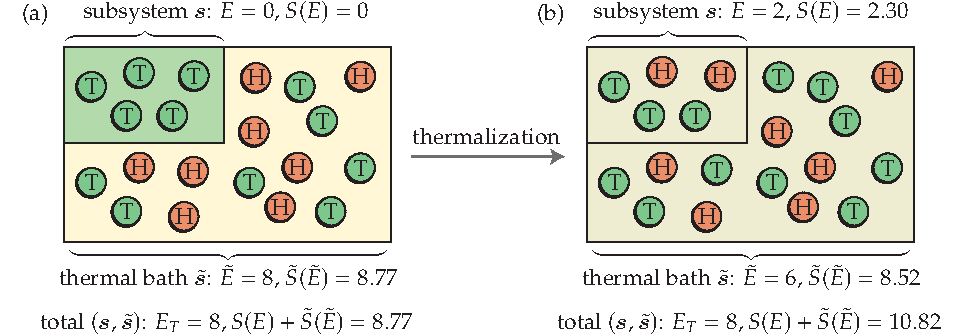
\includegraphics{max_dissertation//chapters//figures//chp1/coin-flip-ensemble.pdf}
    \caption{Thermalization of a subsystem (of coin flips) in contact with a thermal bath. In panel (a) all excited states ("H") are contained in the bath, an unusual configuration with overall entropy $S(E) + \tilde{S}(\tilde{E}) = 8.77$. Panel (b) has a more typical, even arrangement of the excited states, reflected in the higher total entropy $S(E) + \tilde{S}(\tilde{E}) = 10.82$. If the subsystem begins in the ground state (a) it will thus likely thermalize to the equilibrium (b).}
    \label{fig:coin-flip-ensemble}
\end{figure}

To quantify this tendency, we can count the number of overall subsystem-bath configurations~$(\vec{s},\tilde{\vec{s}})$ with subsystem energy~$E$. As in Eq.~\eqref{eq:Omega-E}, there are~$\Omega(E)$ microstates of the subsystem~$\vec{s}$ all share the same energy~$E$. We refer to this collection of microstates as a \emph{macrostate} of the subsystem with energy~$E$. Figure~\ref{fig:coin-flip-entropy} illustrates this grouping of subsystem microstates into macrostates by energy. Macrostates that contain more microstates, those with higher~$\Omega(E)$, are naturally observed more often. We can likewise construct macrostates of the thermal bath~$\tilde{\vec{s}}$ at energies~$\tilde{E}$. Considering the number of ways to arrange the $\tilde{E}$ excited states among the $\tilde{n}$ sites of the bath, there are \begin{align}
    \tilde{\Omega}(\tilde{E}) = \binom{\tilde{n}}{\tilde{E}}
\end{align}
microstates in the bath macrostate of energy~$\tilde{E}$. In many settings the full microstate is not observable, for instance the precise position and velocity of each molecule of a gas. In these settings the macrostate summarizes the pieces of physically relevant information that can be observed, such as the energy or pressure.

\begin{figure}
    \centering
    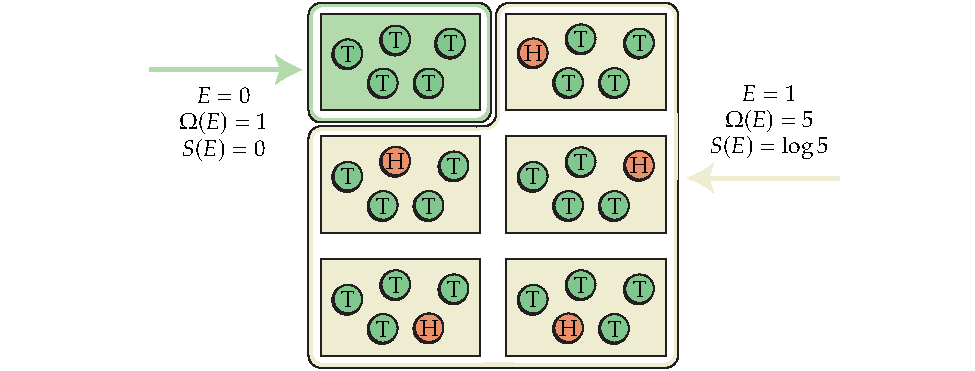
\includegraphics{max_dissertation//chapters//figures//chp1/coin-flip-entropy.pdf}
    \caption{Example microstates of the subsystem~$\vec{s}$ grouped into macrostates by energy~$E$. Only one microstate has~$E = 0$ while five microstates share~$E = 1$, meaning that the higher energy macrostate has higher entropy~$S(E)$. Although each microstate is equally likely, the higher entropy macrostate is more likely to be observed.}
    \label{fig:coin-flip-entropy}
\end{figure}

Since the subsystem macrostate has~$\Omega(E)$ microstates and the bath macrostate has~$\tilde{\Omega}(\tilde{E})$, there are~$\Omega(E)\tilde{\Omega}(\tilde{E})$ unique pairs~$(\vec{s},\tilde{\vec{s}})$ with subsystem energy~$E$ and bath energy~$\tilde{E} = E_T - E$. Since each pair is equally likely to appear in the overall microcanonical ensemble, we thus observe subsystem energy~$E$ with probability \begin{align}
    P(E|E_T) &\propto \Omega(E)\tilde{\Omega}(\tilde{E}) \nonumber \\
    &\propto \Omega(E) \tilde{\Omega}(E_T - E). 
\end{align}
These macrostate multiplicities can also be written using macrostate \emph{entropy}, defined as the logarithm\footnote{More generally defined as~$S = k_B \log \Omega$ where~$k_B \approx 1.38 \text{ J}/\text{K}$ is the Boltzmann constant. The units of this constant are due to the thermodynamic relation Eq.~\eqref{eq:temperature-definition}.} \begin{align}
    S(E) = \log \Omega(E) = \log \binom{n}{E}, \text{ or }\, \tilde{S}(\tilde{E}) = \log \tilde{\Omega}(\tilde{E}) = \log \binom{\tilde{n}}{\tilde{E}}. \label{eq:entropy-microcanonical-definition}
\end{align}
The energy distribution then depends on the overall entropy~$S(E) + \tilde{S}(\tilde{E})$ as \begin{align}
    P(E|E_T) \propto e^{S(E) + \tilde{S}(\tilde{E})}. \label{eq:probability-entropy}
\end{align}
Configurations with higher total entropy are therefore more likely to appear, as calculated in Figure~\ref{fig:coin-flip-ensemble}. This tendency to observe higher entropy states is the content of the 2nd law of thermodynamics: that the entropy of the universe cannot decrease. On such large scales differences in entropy are large, and the probability Eq.~\eqref{eq:probability-entropy} approaches a certainty, a law of physics.

We can similarly compute the distribution of subsystem configurations~$\vec{s}$, not just of its energy~$E$. If we fix the subsystem microstate, valid pairs~$(\vec{s},\tilde{\vec{s}})$ correspond to bath microstates~$\tilde{\vec{s}}$ among the~$\tilde{\Omega}(\tilde{E})$ configurations of the remaining energy. As each pair is equally probable, the subsystem is distributed as \begin{align}
    P(\vec{s}|E_T) &\propto \tilde{\Omega}(\tilde{E}) \nonumber \\
    &\propto e^{\tilde{S}(\tilde{E})}. \label{eq:P-s-E_T}
\end{align}
Unlike the uniform, microcanonical ensemble of the subsystem, certain configurations are now more or less likely based on the entropy of the surrounding bath.

In this picture the \emph{canonical} ensemble is defined by the limit~$\tilde{n} \rightarrow \infty$ of a large thermal bath that can effectively absorb subsystem fluctuations. We further fix the average energy~$p = \tilde{E}/\tilde{n}$ of the thermal bath in this limit, which corresponds to a fixed density of excited states. If we Stirling approximate the binomial coefficient Eq.~\eqref{eq:entropy-microcanonical-definition}, we find the bath's entropy~$\tilde{S}(\tilde{E})$ is proportional to its energy (up to a constant~$C$) as \begin{align}
    \tilde{S}(\tilde{E}) = \beta \tilde{E} + C, \quad \beta = \log \frac{1-p}{p}. \label{eq:tilde-S-tilde-E}
\end{align}
This constant of proportionality~$\beta$ is known as the \emph{inverse temperature} and relates changes in the bath energy~$\tilde{E}$ to changes of entropy~$\tilde{S}$ as \begin{align}
    \frac{\partial \tilde{S}}{\partial \tilde{E}} = \beta = \frac{1}{T}, \label{eq:temperature-definition}
\end{align}
aligning with the usual thermodynamic definition\footnote{This definition ensures that if two thermal baths at temperatures~$T_1 > T_2 > 0$ are brought into contact energy will flow from the higher temperature bath to the lower temperature bath to increase the overall entropy, in keeping with the 2nd law of thermodynamics.} of the temperature~$T$. We will typically assume this temperature is positive and so added energy increases the entropy, although negative temperatures are possible in certain cases such as population inversion in laser physics or the coin flips when~$p > 0.5$.

Comparing to Eq.~\eqref{eq:P-s-E_T}, we then see that the probability of observing any given subsystem~$\vec{s}$ in this canonical ensemble is \begin{align}
    P(\vec{s}|\beta) &\propto e^{\beta \tilde{E}}  \propto e^{-\beta E} \nonumber \\
    &\propto e^{-\beta H(\vec{s})},
\end{align}
where we have used that the total energy~$E_T = E + \tilde{E}$ is conserved. In fact, by similar arguments any system~$\vec{s}$ in thermal equilibrium with a large bath at inverse temperature~$\beta$ follows this same~\emph{Boltzmann distribution} (or "Gibbs distribution")~$P(\vec{s}) \propto e^{-\beta H(\vec{s})}$, which may itself taken as the definition of the canonical ensemble of~$\vec{s}$. When~$T = 0$, $\beta \rightarrow \infty$, the subsystem is stuck in its ground state with the smallest possible energy~$H(\vec{s})$. This aligns with the usual tendency of a physical system towards smaller energy, as a ball rolls down a hill. As the temperature increases and~$T \rightarrow \infty, \beta = 0$, however, the Boltzmann distribution becomes uniform and every subsystem microstate is equally likely independent of its energy.

At finite~$\beta > 0$ between these extremes, the typical thermal configuration may not be the ground state, even though that is the single most likely microstate. Rather, the subsystem is likely to be found in some other macrostate with higher entropy~$S(E)$ as seen in Figure~\ref{fig:coin-flip-ensemble}. Although each individual microstate of this macrostate has smaller probability than the ground state, their greater number makes their macrostate collectively more likely to be observed. This effect can be quantified by revisiting Eq.~\eqref{eq:probability-entropy} for the distribution of energy~$E$. Since the large bath's entropy is proportional to its energy we have \begin{align}
    P(E|E_T) &\propto e^{S(E) + \tilde{S}(\tilde{E})} \propto e^{S(E) + \beta \tilde{E}} \nonumber \\
            &\propto e^{S(E) - \beta E} \propto e^{-\beta F(E)}
\end{align}
where we have defined the \emph{free energy} \begin{align}
    F(E) = E - T S(E).
\end{align}
The most likely energy~$E$ to be observed is therefore the minimum of this free energy. Depending on the temperature~$T$, this may no longer be the ground state energy due to the influence of the entropy~$S(E)$.

To complete the description of the canonical ensemble, we normalize the Boltzmann distribution as \begin{align}
    P(\vec{s}|\beta) = \frac{1}{Z(\beta)}e^{-\beta H(\vec{s})}, \quad Z(\beta) = \sum_{\vec{s}} e^{-\beta H(\vec{s})} \label{eq:boltzmann-distribution}
\end{align}
with the partition function~$Z(\beta)$, a quantity which tells us much about the system in its own right. For example, its logarithmic derivative \begin{align}
    - \partial_\beta \log Z(\beta) &= - \frac{1}{Z(\beta)} \partial_\beta \sum_{\vec{s}} e^{-\beta H(\vec{s})} \nonumber \\
    &= \frac{1}{Z(\beta)} \sum_{\vec{s}} H(\vec{s}) e^{-\beta H(\vec{s})} \nonumber \\
    &= \langle E \rangle \label{eq:average-energy-partition-function}
\end{align}
yields the average energy~$\langle E \rangle$ under the Boltzmann distribution.

If we normalize the Boltzmann distribution of our coin flip system with the partition function~$Z(\beta) = (1-p)^{-n}$, we obtain \begin{align}
    P(\vec{s}|p) &= \frac{1}{Z(\beta)} e^{-\beta H(\vec{s})} \nonumber \\
    &= \frac{1}{(1 - p)^{-n}} e^{-\log \left(\frac{1-p}{p}\right) \, n_H} \nonumber \\
    &= p^{n_H}(1-p)^{n - n_H} \label{eq:coin-flips-thermal}
\end{align}
which we recognize as the model likelihood Eq.~\eqref{eq:coin-flip-likelihood} for biased coin flips with probability~$p$. In this correspondence, we can check that the average energy relation Eq.~\eqref{eq:average-energy-partition-function} of the physical system indeed recovers the expected number of heads \begin{align}
    \langle E \rangle = -\partial_\beta \log Z(\beta) = p n.
\end{align} Unlike the microcanonical ensemble, the number of observed heads~$n_H = E$ can now thermally fluctuate about this expectation via exchange with its surroundings in a manner that exactly reproduces independent coin flips.

This example motivates us to draw a broader analogy between statistics and physics. In Eq.~\eqref{eq:coin-flips-thermal} we described a physical system that reproduces the biased coin flip likelihood, the same distribution of flip outcomes given a fixed parameter~$p$. Often, however, we are interested in the reverse inference problem of understanding the space of likely parameter values~$p$ given a particular observation. Suppose we have a generic model~$P(\vec{x}|\vec{\theta})$ of data~$\vec{x}$ with parameters~$\vec{\theta}$. As discussed in Appendix~\ref{app:statistical-inference}, the posterior distribution of parameters inferred from data~$\vec{x}$ is by Bayes' law \begin{align}
    P(\vec{\theta}|\vec{x}) &= \frac{P(\vec{x}|\vec{\theta})P(\vec{\theta})}{P(\vec{x})}.
\end{align}

For a fixed observation~$\vec{x}$, the corresponding physical system is defined by the Hamiltonian \begin{align}
    H(\vec{\theta}) = -\log P(\vec{x}|\vec{\theta}) \label{eq:energy-posterior-relation}
\end{align}
over the configuration space of possible parameters~$\vec{\theta}$. If we assume a uniform prior~$P(\vec{\theta}) = 1$, the posterior distribution over parameters is proportional to the Boltzmann distribution of this system at unit temperature~$\beta = 1$ \begin{align}
    P(\vec{\theta}|\vec{x}) \propto P(\vec{x}|\vec{\theta}) \propto e^{-H(\vec{\theta})}.
\end{align}
In fact, if we normalize the Boltzmann distribution as \begin{align}
    P(\vec{\theta}|\vec{x}) = \frac{1}{Z(1)} e^{-H(\vec{\theta})},
\end{align}
the partition function~$Z(1)$ is equal to the Bayesian evidence \begin{align}
    Z(1) = \sum_{\vec{\theta}} e^{-H(\vec{\theta})} = \sum_{\vec{\theta}} P(\vec{x}|\vec{\theta}) P(\vec{\theta}) = P(\vec{x}).
\end{align}
Through this correspondence we can explore the posterior distribution of any Bayesian model by simulating the behavior of the analogous physical system. 

This equivalence highlights a subtle philosophical difference between the physical perspective and the common statistical view of these problems. In statistics, particularly in frequentist treatments, we often consider and report the single best-fit parameter of a model that maximizes~$P(\vec{\theta}|\vec{x})$. Physically, this is akin to identifying the ground state configuration with the lowest energy~$H(\vec{\theta})$.

Yet in physics, we are usually more interested in the typical behavior of the system across the entire thermal ensemble rather than the nature of the single most probable microstate. As shown in Figure~\ref{fig:coin-flip-ensemble}, there may be many other less likely yet more entropic configurations that dominate the overall distribution when taken together. In common glass, for example, although the ground state would be an ordered crystalline structure, thermal fluctuations make the typical configuration amorphous, giving the material its signature uniform transparency. Keeping with this perspective, in this work we will consider the full posterior distribution when possible to give a comprehensive picture of system behavior.

For this purpose we employ Markov Chain Monte Carlo (MCMC) methods, a common technique to simulate generic physical systems and so to sample from generic probability distributions. This strategy performs a weighted random walk over configuration space, analogous to thermalization and dispersion in a real system. Returning to our coin flip example, we can consider how in Figure~\ref{fig:coin-flip-ensemble} the subsystem dynamically evolves. If our subsystem~$\vec{s}$ begins in a the low entropy ground state (a), through the jostling of the coins the system will naturally tend towards a typical, high entropy configuration (b). Yet physically this transition is not instantaneous. For instance, gas molecules kinetically bump into each other and gradually disperse throughout their enclosure. We use Markov chain methods to simulate coin flip thermalization as a process that occurs one coin flip at a time. 

A Markov chain walks through configuration space in discrete increments of time. At each step the Markov chain \emph{transitions} from one state at time~$t$ to another state at slightly later time~$t + \Delta t$. This is a random walk, where a move from state~$\vec{s}$ to~$\vec{s}'$ is made with probability $P(\vec{s} \rightarrow \vec{s}')$. Under mild conditions on the transition probabilities, this Markov chain will converge to some equilibrium distribution~$P(\vec{s})$. If the states of the Markov chain are distributed according the equilibrium~$P(\vec{s})$, the final~$\vec{s}'$ after the chain move~$\vec{s} \rightarrow \vec{s}'$ will by definition share the equilibrium distribution \begin{align}
    P(\vec{s}') = \sum_{\vec{s}}P(\vec{s})P(\vec{s} \rightarrow \vec{s}'). \label{eq:MCMC-stability}
\end{align}
We are then left with the problem of constructing a Markov chain which has the particular equilibrium distribution~$P(\vec{s})$ we are interested in.

A simple and ubiquitous way to establish such a chain is known as the \emph{Metropolis-Hastings algorithm}. Each step in this Markov chain consists of two parts. First, a move to a new state is \emph{proposed} given the current state. Second, that move is either \emph{accepted} and the chain moves to the new state, or it is \emph{rejected} and the chain remains at its current state. If we propose moves with transition probabilities~$P_{\text{prop}}(\vec{s} \rightarrow \vec{s}')$, we accept each proposal with probability \begin{align}
    P_{\text{acc}}(\vec{s} \rightarrow \vec{s}') = \text{min}\left(1, \frac{P(\vec{s}')P_{\text{prop}}(\vec{s}' \rightarrow \vec{s})}{P(\vec{s})P_{\text{prop}}(\vec{s} \rightarrow \vec{s}')}\right).
\end{align}
We will often use symmetric proposals where~$P_{\text{prop}}(\vec{s} \rightarrow \vec{s}') = P_{\text{prop}}(\vec{s}' \rightarrow \vec{s})$, for which this acceptance probability simplifies to \begin{align}
    P_{\text{acc}}(\vec{s} \rightarrow \vec{s}') = \text{min}\left(1, \frac{P(\vec{s}')}{P(\vec{s})}\right) = \text{min}\left(1, e^{\beta(H(\vec{s}) - H(\vec{s}'))}\right).
\end{align} 
In terms of the system energy~$H(\vec{s})$, we see that the algorithm will always accept changes that decrease the energy, and occasionally moves that increase it, an emulation of how the real system evolves.

From this two-step process the overall Markov chain transition probabilities are then distinguished by if they increase or decrease the probability as \begin{align}
    P(\vec{s} \rightarrow \vec{s}') = \begin{cases}
        P_{\text{prop}}(\vec{s} \rightarrow \vec{s}') & P(\vec{s}') \geq P(\vec{s}), \vec{s} \not= \vec{s}'\\
        P_{\text{prop}}(\vec{s} \rightarrow \vec{s}')\frac{P(\vec{s}')}{P(\vec{s})} & P(\vec{s}') < P(\vec{s})\\
        P_{\text{prop}}(\vec{s} \rightarrow \vec{s}) + \sum_{\vec{s}' < \vec{s}} P_{\text{prop}}(\vec{s} \rightarrow \vec{s}') \left[1 - \frac{P(\vec{s}')}{P(\vec{s})}\right]& \vec{s}' = \vec{s}
    \end{cases}
\end{align}
where sum in the case~$\vec{s}' = \vec{s}$ accounts for all the rejected proposals to states~$\vec{s}'$ with probability~$P(\vec{s}') < P(\vec{s})$. Summing over these cases, now of states~$\vec{s}$ that can produce a state~$\vec{s}'$, we can check the stability condition Eq.~\eqref{eq:MCMC-stability} as \begin{align}
    \sum_{\vec{s}} P(\vec{s})P(\vec{s} \rightarrow \vec{s}') &= \sum_{\vec{s} < \vec{s}'} P(\vec{s}) P_{\text{prop}}(\vec{s} \rightarrow \vec{s}') + \sum_{\vec{s} > \vec{s}'} P(\vec{s}) \frac{P(\vec{s}')}{P(\vec{s})}P_{\text{prop}}(\vec{s} \rightarrow \vec{s}') \nonumber\\
    &+ P(\vec{s}')P_{\text{prop}}(\vec{s}' \rightarrow \vec{s}') + P(\vec{s}') \sum_{\vec{s} > \vec{s}'} P_{\text{prop}}(\vec{s}' \rightarrow \vec{s})\left[1 - \frac{P(\vec{s})}{P(\vec{s}')}\right] \nonumber\\
    &= P(\vec{s}')\sum_{\vec{s}} P_{\text{prop}}(\vec{s} \rightarrow \vec{s}') = P(\vec{s}').
\end{align}

Therefore the desired distribution is a fixed point of the Metropolis-Hastings algorithm, regardless of the choice of proposals~$P_{\text{prop}}(\vec{s} \rightarrow \vec{s}')$. However, being a Markov chain, there is still a clear correlation between subsequent steps in the random walk. Only after a typical number of Markov chain known as the \emph{mixing time} are the samples meaningfully independent. Therefore to efficiently obtain independent samples from the distribution, to for example compute expectations, the mixing time should be as small as possible. The form these proposals take can considerably impact the mixing time, and clever choices are often needed to make Monte Carlo methods tractable.

A common choice of proposal for discrete settings like this is to consider \emph{single site flips} where we choose a random site~$i$ and flip it from heads to tails, $s_i = 1 \mapsto 0$  or vice versa. An advantage to this local change is that the resulting chance in the probability (or energy) is small and therefore likely to be accepted. If a entirely new global configuration is drawn uniformly at random, it likely has a much lower probability (or higher energy) than the current sample, and so will likely be rejected and waste an iteration of the algorithm.

\begin{figure}
    \centering
    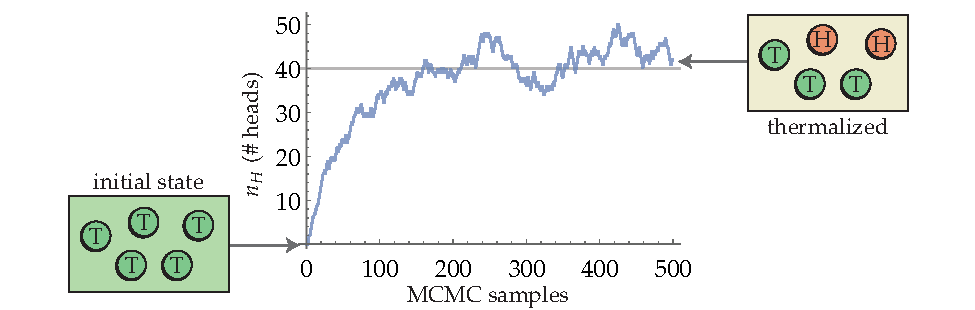
\includegraphics{max_dissertation//chapters//figures//chp1/MCMC-coin-flip.pdf}
    \caption{Trajectory of the Metropolis-Hastings MCMC algorithm to thermalize a system of 100 coin flips. The system begins in the ground state where~$n_H = 0$. The average value~$n_H = 40$ is highlighted. Once the Markov chain has thermalized, the samples are indicative of this average value.}
    \label{fig:MCMC-coin-flip}
\end{figure}

If we apply this to our simple coin flipping example, Figure~\ref{fig:MCMC-coin-flip} shows how the number of flips changes over the course of the Metropolis-Hastings algorithm. We can observe that although the system starts in a configuration not particularly representative of the equilibrium distribution, after many iterations the Markov chain thermalizes the state. Although this is a fairly simple distribution, one we could sample directly, the flexibility of MCMC allows us apply it to far more complex distributions to draw inferences. In doing this, however, we must be careful to ensure that the Markov chain has adequately converged. If samples are interpreted too early in the algorithm, results will be skewed by the initial state, as in the initial samples of Figure~\ref{fig:MCMC-coin-flip}.

These Monte Carlo methods are very powerful, and are the workhorse of the statistical inferences made in this thesis. In order to apply these methods to their fullest, we can further augment the Metropolis-Hastings algorithm by performing \emph{parallel tempering} to reduce the mixing time of the Markov chains and \emph{thermodynamic integration} to compute the Bayesian evidence in a manner analogous to how such methods are used to compute the physical free energy. 